\documentclass[a4paper,11pt]{jarticle}
\usepackage{ics-thesis}
\usepackage{amssymb}
\usepackage[dvipdfmx]{graphicx}
\usepackage{subcaption}
\pagestyle{bachelorthesis}    % 卒論・規定の.styファイルを使う場合
%
\title{サイボーグインセクトによる迅速な被災者発見のための自己組織型移動制御手法の提案と評価}
\author{北浦 直}
\supervisor{若宮 直紀 教授}
\deadline{2019年2月12日}
%
\begin{document}
	\titlepage    % 規定の.styファイルを使う場合
	\abstract     % 規定の.styファイルを使う場合
	%%%%%%%%%%%%%%%%%%%%%
	% 内容梗概本文
	%%%%%%%%%%%%%%%%%%%%%
	\keyword
	%%%%%%%%%%%%%%%%%%%%%
	% キーワード
	%%%%%%%%%%%%%%%%%%%%%
	\tableofcontents    % 目次
	%
	%%%%%%%%%%%%%%%%%%%%%
	% 本文
	%%%%%%%%%%%%%%%%%%%%%
	%
	\section{はじめに}
	災害が起きた場合,倒壊した建物内に被災者が取り残されることが起こりうる.
	倒壊した建物内に捕らわれた被災者の探索において,現在は災害救助犬やスコープカメラなどの人間の能力を補助するような手法が広く使われている\cite{USR}.
	しかし,倒壊した建物内は狭い隙間であったり,アスベストやほこり,危険物の存在により人間や災害救助犬が入れないような環境である可能性がある\cite{environment}.
	また,救助活動の中で2次災害が起きてしまう事例も少なくない.
	そこで,現在の探索手法では探索できないような狭い空間を探索可能で,探索中の2次災害の危険性を低くすることができるサイボーグインセクトを用いた被災者探索の研究がなされている\cite{CyborgInsect}.

	サイボーグインセクトを被災者探索に活用するための研究としてCINEMa(Cyborg Insect Networks for Exploration and Mapping)があげられる\cite{CINEMa}.
	この研究の中では,サイボーグインセクトへ制御を与えて任意の方向へ向かわせたり,サイボーグインセクトが位置推定をするためのアルゴリズムの実験がされていたりする.
	しかし,CINEMaはがれきなどが散乱するような悪条件下における被災者探索に必要な構成要素の説明は行われているが,それらを用いて被災者探索を効率的に行うための制御手法などは提案されていない.
	つまり,群で探索しているにも拘らず複数個体がほぼ同一の場所を探索することで空間全体を探索するのにかかる時間が増加してしまう恐れがある.
	
	そこで,サイボーグインセクトの群れが効率的に空間全体を探索できるような制御を与えたい.
	しかし,救助者は倒壊した建物内の詳細な環境を知ることはできないため,救助者から細かい操作を行うことは不可能である.
	よって,サイボーグインセクト自身が得られる情報をもとに自律的に制御を行い空間探索を行う必要がある.
		
	また,自律的な制御アルゴリズムの1つであるフロッキングという手法がある.
	フロッキングとは,周囲の個体に対して,衝突回避,中心移動,方向調整の3つの動作をとることで複数個体が群れとなって動くようなアルゴリズムである\cite{flocks}.
	文献\cite{flockingsearch}のようにフロッキングを被災者探索に適用される研究が行われているが,フロッキングをサイボーグインセクトに適用して被災者探索を実現している研究はなされていない.
	また,レスキューロボットなどのフロッキング制御とは違い,サイボーグインセクトに与えるフロッキングの制御は生物に電気信号を流すためできるだけ頻度が低いことが望ましい.
	
	そこで,本研究ではCINEMaで提案されているようなサイボーグインセクトの群れに対するフロッキング制御手法の提案を行う.サイボーグインセクトのモデルと断続的な制御をシミュレーション上に実装し,制御されていない場合の探索と制御された場合の探索を比較する.ここでは,サイボーグインセクトに対する断続的なフロッキング制御でも探索にかかる時間の短縮ができることを確認する.
	
	以降,第\ref{sec:CyborgInsect}章では,本研究に用いるサイボーグインセクトに関する説明を行い,第\ref{sec:flocking}章でフロッキング動作の説明を行う.第\ref{sec:algorithm}章でサイボーグインセクトが制御をされていない場合の動作について述べ,第\ref{sec:control}でサイボーグインセクトへ与える制御について述べる.第\ref{sec:result}章では実験結果について述べる.第\ref{sec:last}章では本研究のまとめと今後の課題について述べる.
	\section{サイボーグインセクト}
	\label{sec:CyborgInsect}
	%関連研究→この研究で想定するスペック
	この章では,本研究で考えるサイボーグインセクトの概要と,サイボーグインセクトに取り付けられる機材,本研究でのサイボーグインセクトに関する条件の説明を行う.
	
	サイボーグインセクトとは,文献\cite{CyborgInsect}で示されているような,機械を埋め込み人間が操作できるようにした昆虫に計器類を乗せて被災者探索を可能にしたものを指す.
	このサイボーグインセクトの特徴として,昆虫の移動能力がそのまま使えるため,壁や天井も移動できて,かつ狭い場所にも侵入可能という探索できない場所の少なさが挙げられる.
	また,同等な移動能力を持つレスキューロボットに比べると1匹当たりの値段が安く済むため,探索に使える群の数を多くできることも利点である.
	
	サイボーグインセクトには,神経刺激による移動制御,センシング,サイボーグインセクトの位置推定、および救助者や周りのサイボーグインセクトとの通信のための機材が乗せられている.
	
	サイボーグインセクトに対する制御は,壁で仕切られた迷路の指定された経路を通るなどの実験を通して,サイボーグインセクトの本来の動きによらず移動の制御操作ができることを示している\cite{CINEMa}.
	
	文献\cite{CINEMa}の中で,センシングのために様々なセンサをサイボーグインセクトに積載すると示されている.具体的に挙げられていたのは,3方向の加速度計,ジャイロスコープ,磁力計,指向性マイクと全指向性マイク,ブザーとスピーカー,赤外線検知器,ガス検知器がサイボーグンセクトへ取り付ける機材として挙げられていた.
	
	被災者のセンシングに関して,複数のマイクでの音の強度を比較することで音源方向の特定をしてサイボーグインセクトから見た被災者の方向を特定することができていた.
	また,サイボーグインセクトに取り付けられたマイクとスピーカーを利用することによって,サイボーグインセクト自身の位置推定を行っていた.
	
	今研究では,神経刺激による移動制御は十分に可能として考える.被災者や障害物のセンシングは,半径2m以内ならできると考え,距離精度は10cm単位,角度の精度は10度単位として考える.
	また,サイボーグインセクト同士の通信可能範囲は5mとする.
	
	\section{迅速な被災者発見のための制御手法}
	\label{sec:control}
	\subsection{制御の概要}
	%全体に広がってほしい,間欠的な制御制御を行うこと
	被災者の数やいる場所がわからない中での被災者探索は,空間全体を探索する必要がある.
	そこで,空間全体を迅速に探索するために,サイボーグインセクトの群れが空間全体に分散することを考えた.
	空間全体に分散したサイボーグインセクトの群れが,それぞれの個体の周辺を探索することで,探索の冗長性を少なくして迅速に空間全体を探索できる.
	
	また,\ref{sec:CyborgInsect}章で説明したサイボーグインセクトの条件より,消費電力やサイボーグインセクトへの負担の軽減が物理的な制約として存在する.
	そこで,サイボーグインセクトに対しては連続な制御を行うことなく,間欠的に制御を行うことを考える.
	\subsection{フロッキング}
	%一般的なモデルの説明
	\label{sec:flocking}
	この章では,フロッキングについて説明する.
	フロッキング制御は,ロボット群への自己組織型制御として被災者探索などに使われているアルゴリズムである.
	フロッキング制御では,ロボット群が相互作用によって一定の距離を保ち,群れとして行動することで探索の冗長性を軽減している.
	そこで,本研究では,フロッキング制御の衝突回避の式を用いることを考えた.
	
	フロッキングとは,自然界の鳥や魚の群れで見られるような,複数の個体が同じ目標に向かい連動して動くような行動である.
	この自然界で見られる行動を限定された範囲のセンシング能力とコミュニケーションにより再現したモデルが知られている.
	文献\cite{steering}では衝突回避,中心移動,方向調整の3つの動作によりフロッキングのモデル化を行っている.それぞれの動きは図\ref{fig:flocking}のようにあらわされる.
	
	\begin{figure}
		\begin{minipage}{0.3\linewidth}
			\centering
			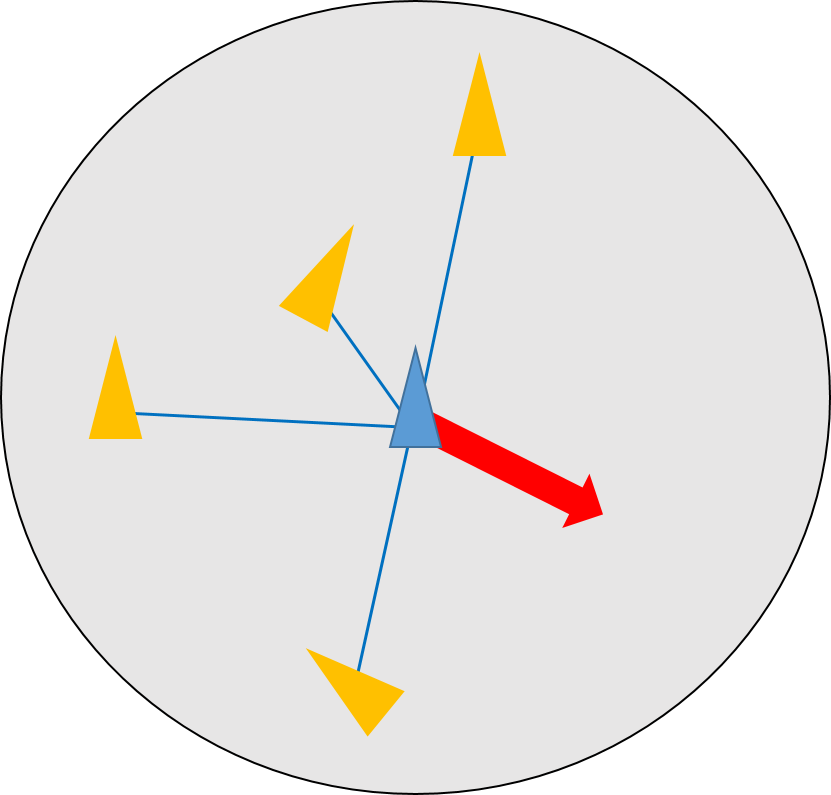
\includegraphics[width=0.9\linewidth]{png/separation.png}
			\subcaption{衝突回避}
		\end{minipage}
		\begin{minipage}{0.3\linewidth}
			\centering
			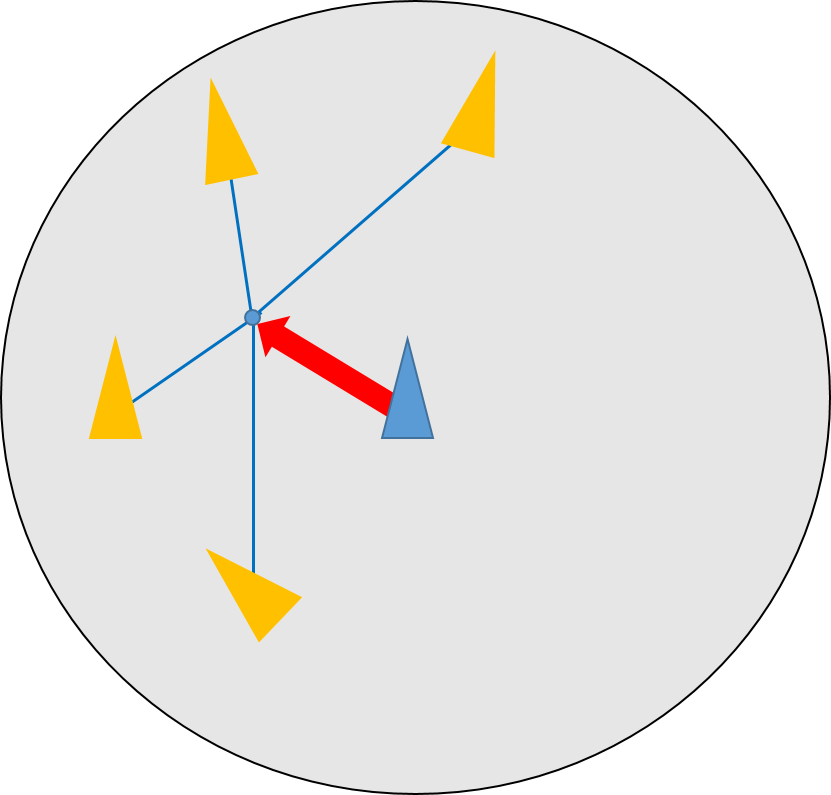
\includegraphics[width=0.9\linewidth]{png/cohesion.png}
			\subcaption{中心移動}
		\end{minipage}
		\begin{minipage}{0.3\linewidth}
			\centering
			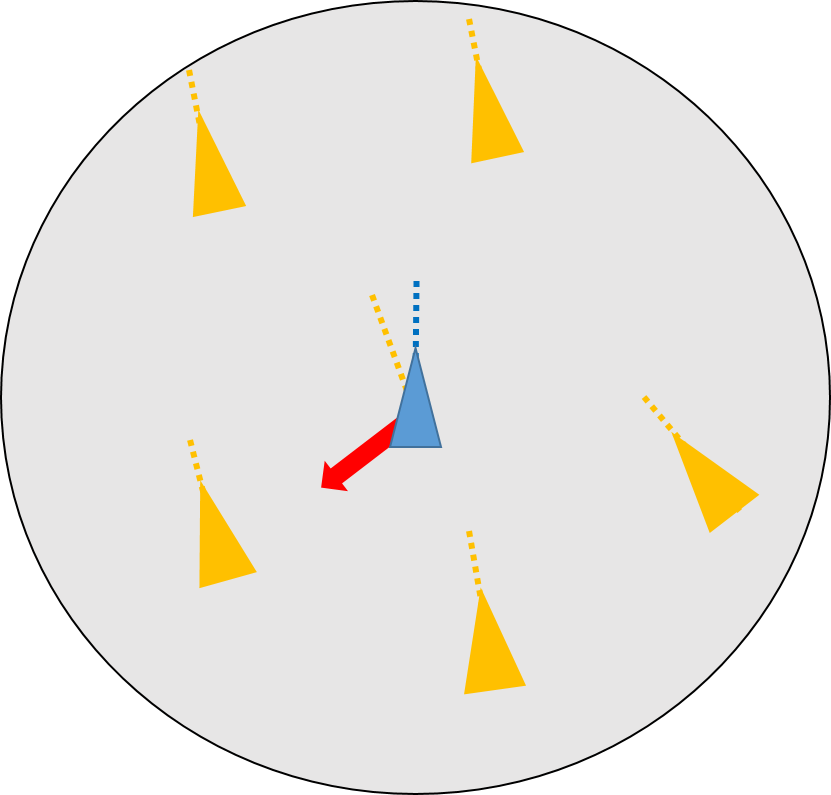
\includegraphics[width=0.9\linewidth]{png/alighnment.png}
			\subcaption{方向調整}
		\end{minipage}
		\caption[フロッキング]{フロッキングの動作}
		\label{fig:flocking}
	\end{figure}
	
	衝突回避の動作により,フロッキングを行っている個体群はそれぞれの距離を一定以上に保つことができる.衝突回避のために,まず,検知できる範囲の中にいる他の個体を探す.その後,検知できる範囲にいた個体から自分までのベクトルを計算し,正規化を行い,さらに自分と見つけた個体との距離でそのベクトルを割る.これを検知できる範囲内の周りの個体すべてに繰り返すことで衝突回避の動作のためのベクトルが得られる.
	
	中心移動の動作によって,フロッキングを行っている個体群は離れすぎることなく群れとしての形を保つことができる.中心移動のために,まず、衝突回避と同様に検知できる範囲の中にいる個体を探す.そして自分を除いた検知できる範囲の中にいる個体群の重心を計算して,その重心へのベクトルを計算する.
	
	方向調整の動作によって,フロッキングを行っている個体群は同じような速度,向きで動くことができる.方向調整のために,衝突回避と同様に検知できる範囲の中にいる個体を探す.そして,それらの個体群の速度の平均を求め,自分の速度との差を求める.この速度の差が方向調整のためのベクトルとなる.
	
	最後に,上記3つのベクトルからフロッキングを行うためのベクトルを求める.この時に,それぞれを足すだけでもフロッキングとして動く場合も存在するが,基本的には,それぞれを正規化したのちに,重み付け係数を用いてスケーリングすることが有用であるといわれている.
	
	さらに,上記のフロッキングの基本的な動作に加えて,障害物ある環境でのフロッキングを考えた研究もなされている\cite{obstacle}.
	また,フロッキングを用いて被災者探索を行う研究も存在する.
	例えば,文献\cite{exploration}では群ロボットによる空間探索において,フロッキングを用いて各ロボットの探索領域の重複の軽減を行っている.
	\subsection{斥力にもとづく進行方向の決定}
	この章では,サイボーグインセクトの群れが空間全体に広がるための制御の内容について説明する.
	フロッキング制御の衝突回避の式を用いて,サイボーグインセクトの群れが空間全体に広がるような制御を考える.
	\section{シミュレーションによる評価}
	この章では,\ref{sec:control}章で提案した制御手法をシミュレーションで実行し,その結果を評価する.
	\subsection{シミュレーション条件}
	この章では,シミュレーションに関する条件などを示す.
	
	まず,本研究のシミュレーションにおいては,倒壊した工場内の被災者探索を行うシナリオを考える.
	そこで,空間の広さは経済産業省の工場立地動向調査平成29年度より,工場立地面積の平均が1228haだったため,80m$\times$150m$\times$4mとすることにした.
	また,今回のシミュレーションでは簡単のために空間を立方体の集合として考え,ボクセルベースで実装した.立方体のサイズは1辺10cmとしている.%理由は?
	
	また,サイボーグインセクトについて,探索を行うサイボーグインセクトの数は100匹とする.被災者を検知できる範囲は半径2mで,障害物の有無を検知できる範囲も同様である.
	サイボーグインセクト同士の通信範囲は5mとする.通信の頻度は,制御周期$T$と同じとする.
	\subsection{評価指標}
	評価指標として,空間探索率を導入する.ここでの空間探索率とは,空間全体のボクセル数に対する探索したボクセル数の割合を指す.
	また,シミュレーションの各ステップにおいて,各サイボーグインセクトの被災者を検知できる範囲内にあるボクセルを探索されたと判定する.
	%空間探索率がどうなればいいのか
	\subsection{サイボーグインセクトのモデル}
	\label{sec:algorithm}
	この章では,シミュレーションに用いるサイボーグインセクトのモデルについて説明を行う.
	サイボーグインセクトのモデルは,制御を行わない場合のモデルと,提案した制御手法を受けるモデルの2種類を考案した.
	\subsubsection{制御されていないサイボーグインセクトのモデル}
	\label{sec:not_control}
	この章では,サイボーグインセクトが制御を受けていない場合の動きのモデルについて説明を行う.
	
	サイボーグインセクトが制御されていない場合の動きについて,基本的に面上を動いているときは直進を続け,面と面が構成する境界線を検知したらその境界線に従う確率が高い動きだと考えた.この時に,面と面のなす角度や重力方向などでそれぞれの動きを選択する確率が変動すると思われる.
	そこで,この考えを満たすようなサイボーグインセクトのモデルを考案した.
	
	このサイボーグインセクトのモデルのアルゴリズムをフローチャートにしたものを図\ref{fig:algorithm}に示す.
	\begin{figure}
		\centering
		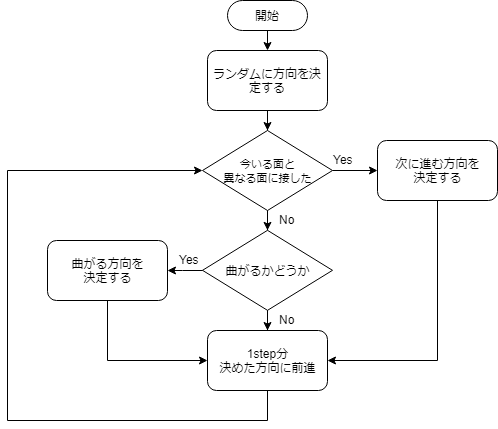
\includegraphics[width=0.7\linewidth]{png/Untitled.png}
		\caption[アルゴリズムのフローチャート]{制御されていないサイボーグインセクトのアルゴリズムのフローチャート}
		\label{fig:algorithm}
	\end{figure}

	\subsubsection{提案手法による拡張}
	この章では,\ref{sec:not_control}章で説明したモデルに対して,拡張を行う.
	提案する制御手法は,\ref{sec:control}章で記述した手法である.
	\subsection{シミュレーション結果と考察}
	\section{おわりに}
	\label{sec:last}
	本報告では,サイボーグインセクトのモデルを作成し,そのモデルにおいて迅速な被災者探索を目的としたサイボーグインセクト群への自律型制御手法の提案・評価を行った.その結果,断続的な制御であっても探索の冗長性を軽減し,探索にかかる時間を短くすることができることが分かった.
	
	今後の課題として,今回用いたシミュレーションでは空間をボクセルベースで実装しているため,より現実的な倒壊した建物内の状況で提案手法が有用であるのかの調査を行う必要がある.

%	\bibliographystyle{unsrt}
%	\bibliography{document}
	\begin{thebibliography}{99}
		%%%%%%%%%%%%%%%%%%%%%
		% 参考文献リスト
		%%%%%%%%%%%%%%%%%%%%%
		\bibitem{USR} Wen-Ta Chiu,Jeffrey arnold,Yaw-Tang Shih,Kuang-Hua Hsiung,Hsueh-Yun Chi,Chia-Huei Chiu,Wan-Chen Tsai,and William C.Huang. A Survey of International Urban Search-and-rescue Teams following the Ji Ji Earthquake. \textit{Disasters},vol.26,no.1,2002,pp.85-94
		\bibitem{environment}Casper J and Murphy R R. Human-robot interactions during the robot-assisted urban search and rescue response at the world trade center.\textit{Systems,Man, and Cybernetics, PartB:Cybernetics,IEEE Transactions on,33(3)},2003,367-385
		\bibitem{CyborgInsect}Alper Bozkurt,Robert F.Glimour,Ayesa Sinha,David Stern,and Amit Lal. Insect-Machine Interface Based Neurocybernetics. \textit{IEEE Trans Biomedical Eng.},vol.56,no.6,2009,pp.1727-1733
		\bibitem{CINEMa}Alper Bozkurt,Edgar Lobaton,and Mihail Sichitiu.A Biobotic Distributed Sensor Network for Under-Rubble Search and Rescue.\textit{Computer},vol.49,no.5,pp.38-46,2016
		\bibitem{flocks}Craig Reynolds. Flocks, herds and schools: A distributed behavioral model. \textit{ACM SIGGRApH Computer Graphics},vol.21,1987,pp25-34
		\bibitem{flockingsearch}M.G.C.A.Cimino,A.Lazzero,G.Vaglini. Combining stgmergic and flocking behaviors to coordinate swarms of drones performing target search. \textit{International Conference on Information,Intelligence,Systems and Applications},2015,pp.1-6
		\bibitem{steering}Craig Reynolds. Steering behaiviors for autonomous characters.In \textit{Proceedings of Game Developers Conference},pages 763-782,1999.
		\bibitem{obstacle}Ali E.Turgut,Hande Celikkanat,Fatih Gokce,and Erol Sahin. Self-organized flocking in mobile robot swarms. \textit{Swarm Intelligence},vol.2,pp97-120,2008
		\bibitem{exploration}Noury Bouraqadi,and Arnaud Doniec. Flocking-Based Multi-Robot Exploration. \textit{Conttol Architectures of Robots}.2009
		\bibitem{speed}J.M. Camhi, E.N. Johnson. HIGH-FREQUENCY STEERING MANEUVERS MEDIATED BY TACTILE CUES: ANTENNAL WALL-FOLLOWING IN THE COCKROACH. \textit{Journal of Experimental Biology},pp.631-643,1999
		\bibitem{flocking-robot}Ali E.Turgut, Hande Celikkanat, Faith Gokce, and Erol Sahin. Self-organized flocking in mobile robot swarms.
		\bibitem{rubble}小野里 雅彦, 増田 寿信, 毛利 健二, 伊達 宏昭, 田中 文基. がれき内部空間の構造分析に関する研究.\textit{図学研究},pp.45-48,2008
		
	\end{thebibliography}
\end{document}